\newcommand{\paperdoi}{10.5281/zenodo.18810431}
\newcommand{\papertitle}{Phase Locking and Discrete Mode Selection in Closed Circulation Loops}
\newcommand{\papershorttitle}{Phase Locking in Circulation Loops}
\newcommand{\paperorcid}{0009-0006-1686-3961}
\newcommand{\paperemail}{info@omariskandarani.com}
\newcommand{\papercity}{Groningen}
\newcommand{\papercountry}{The Netherlands}
\newcommand{\paperkeywords}{Delay differential equations, Phase locking, Nonlinear dynamical systems, Stability analysis, Spectral discreteness, Circulating feedback systems}


%=========================================
% % PREAMBLE, PACKAGES AND DOCUMENT CONFIGURATION
%=========================================
\documentclass[pdflatex,sn-mathphys-num]{sn-jnl}
\usepackage{graphicx}%
\usepackage{multirow}%
\usepackage{amsmath,amssymb,amsfonts,bm}
\usepackage{amsthm}%
\usepackage{mathrsfs}%
\usepackage[title]{appendix}%
\usepackage{xcolor}%
\usepackage{textcomp}%
\usepackage{manyfoot}%
\usepackage{booktabs}%
\usepackage{algorithmicx}%
\usepackage{listings}%

\usepackage{siunitx}
\usepackage[T1]{fontenc}
\usepackage[utf8]{inputenc}
\usepackage{pgfplots}
\pgfplotsset{compat=1.18}
\usetikzlibrary{pgfplots.groupplots}


%=========================================
% Start Document - Title Page
%=========================================
\raggedbottom
\begin{document}

    \title[\papershorttitle]{\papertitle}

    \author*[1]{\fnm{Omar} \sur{Iskandarani}}
    \email{\paperemail}

    \affil*[1]{\orgname{Independent Researcher}, \orgaddress{\city{\papercity}, \country{\papercountry}}}

    \abstract{
        Closed circulation loops with finite propagation time constitute a broad and generic class of delayed feedback systems encountered across fluid dynamics, optics, electronics, and wave physics \cite{Erneux2009,Hale1993,Diekmann1995,GlassMackey1988,Ikeda1979}.
        We show that such loops admit discrete, dynamically selected phase--locked states even when governed by fully continuous classical dynamics \cite{Pikovsky2001,Kuramoto1984,Strogatz2003book}.
        Using a minimal delayed phase oscillator as a canonical model, we demonstrate that finite circulation time enforces multistable phase--locking conditions.

        The resulting phase--locked solutions form a countable family of circulation modes.
        By analyzing the characteristic equation of the differenced delayed dynamics, we prove that stability filtering eliminates the odd-indexed branches in the strong-feedback regime.
        This yields an evenly spaced, integer-indexed subset of dynamically stable frequencies.

        The asymptotic spacing coincides with that of periodic boundary quantization for a wave on a loop \cite{Zettl2005,Griffiths2018}, but arises here purely as a set of attractors of a nonlinear delay differential equation.
        This work therefore provides a deterministic classical route to mode discreteness in circulating systems without invoking microscopic quantization.
    }

    \keywords{\paperkeywords}

    \maketitle


%=========================================
% Title Page End
%=========================================

    \section{Introduction and Physical setting}

        The origin of discrete spectra in physical theories is conventionally traced to either spatial boundary conditions in wave mechanics (Sturm--Liouville problems) or axiomatic quantization rules in microscopic physics \cite{Zettl2005,Griffiths2018}. In macroscopic, continuous dynamical systems, however, discreteness is not typically an intrinsic property. A broadly applicable question in theoretical physics is whether purely continuous, classical dynamics can autonomously generate a discrete, integer-indexed spectrum of states without invoking geometric spatial confinement or non-commuting operators \cite{Erneux2009,GlassMackey1988}.

        In this work, we address this question by investigating the role of temporal nonlocality in circulating systems. Consider a continuous excitation propagating on a closed loop of fixed geometric length $L$ with characteristic transport speed $v$. The closed geometry defines a finite circulation or round--trip time
        \begin{equation}
            \tau = \frac{L}{v},
            \label{eq:tau}
        \end{equation}
        which represents the time required for information carried by the excitation to return to its point of origin. The internal state of the excitation is characterized by a phase variable $\phi(t)$ that evolves continuously in time and plays the role of an intrinsic clock associated with the circulating structure.

        Because information propagates around the loop in a finite time $\tau$, the local phase evolution at time $t$ is influenced by the phase state that completed one full circulation at time $t-\tau$. This feedback is not externally imposed but is a direct consequence of loop closure and finite propagation speed. As a result, delayed self--interaction is an unavoidable and intrinsic feature of closed circulation systems, regardless of their microscopic realization \cite{Hale1993,Diekmann1995,Erneux2009}.

    \section{Minimal delayed phase model}
        A minimal classical description capturing this delayed feedback is given by a delayed phase oscillator of the form
        \begin{equation}
            \dot{\phi}(t) = \Omega_0 + K \sin\big(\phi(t-\tau) - \phi(t)\big),
            \label{eq:delayed_oscillator}
        \end{equation}
        where $\Omega_0$ is the natural angular frequency associated with unperturbed circulation, $K$ is a real coupling constant encoding the strength of feedback between successive circulations, and $\tau$ is the circulation delay. This equation represents a continuous, deterministic dynamical system with finite propagation time and smooth nonlinearity.

        Importantly, the model contains no quantization postulates, no discrete variables, and no topological constraints. All discreteness that emerges from the dynamics is therefore generated internally by classical delay--induced feedback. Variants of this equation appear naturally in delayed oscillators, phase--locked loops, and wave propagation in closed resonant structures \cite{Erneux2009,Earl2003,Gardner2005,Ikeda1979}.

    \section{Phase--locked solutions}

        Uniformly rotating, or phase--locked, solutions are sought in the form
        \begin{equation}
            \phi(t) = \Omega t + \phi_0,
            \label{eq:ansatz}
        \end{equation}
        where $\Omega$ is a constant rotation rate and $\phi_0$ is arbitrary.
        Substitution into Eq.~\ref{eq:delayed_oscillator} yields
        \begin{equation}
            \Omega = \Omega_0 - K \sin(\Omega\tau).
            \label{eq:self_consistency}
        \end{equation}

        When $\beta=K\tau$ is small, Eq.~\ref{eq:self_consistency} admits a single solution.
        For sufficiently large delay or feedback strength, multiple branches emerge.

        In this work, we define the \emph{dynamically selected spectrum} as the set
        \begin{equation}
            \mathcal{S} :=
            \left\{
            \Omega \in \mathbb{R} \;\middle|\;
            \Omega \text{ satisfies Eq.~\ref{eq:self_consistency} and is linearly stable}
            \right\}.
            \label{eq:frequency_set}
        \end{equation}

        Thus the term ``spectrum'' refers to the discrete set of attracting phase--locked frequencies of the delay equation, not to eigenvalues of a linear operator.

    \section{Stability and mode selection}
        Not all phase--locked solutions are dynamically stable. Linear stability analysis of delay differential equations reveals that stability depends on the characteristic equation obtained from linearization about the phase--locked orbit \cite{Hale1993,Diekmann1995,Erneux2009}. Linear stability analysis reveals that stability depends on the derivative of the right--hand side of the self--consistency relation \ref{eq:self_consistency} with respect to $\Omega$. Only solutions satisfying appropriate slope conditions correspond to attracting states of the delayed dynamics.

        As a consequence, the loop does not support a continuum of circulation frequencies. Instead, it dynamically selects a discrete subset of stable phase--locked modes. Transitions between these modes require the loss of stability of one branch and the capture by another, typically through bifurcations as parameters such as $K$ or $\tau$ are varied. Mode discreteness therefore arises as a direct outcome of classical stability selection rather than any imposed quantization rule.

    \section{Delay-Induced Discreteness vs. Boundary Quantization}

        The emergence of discrete spectra in physical theories is traditionally attributed to either geometric boundary conditions or canonical quantization postulates \cite{Zettl2005,Griffiths2018}.
        In classical wave mechanics, discrete modes arise as solutions to Sturm-Liouville eigenvalue problems, where spatial confinement enforces kinematic constraints \cite{Zettl2005}.
        In quantum mechanics, discreteness is introduced axiomatically via non-commuting observables or single-valuedness requirements of the wavefunction on multiply connected domains \cite{Griffiths2018}.

        By contrast, the mechanism presented here shows that discreteness may arise from the continuous temporal dynamics of delayed self-interaction, without invoking spatial confinement or operator commutation relations.

        In a canonical boundary value problem, such as a particle in a one-dimensional box or a closed optical cavity of length $L$, the spatial constraint $\psi(0)=\psi(L)$ enforces the kinematic condition
        \begin{equation}
            k_n L = 2\pi n, \qquad n\in\mathbb{Z},
            \label{eq:kinematic_condition}
        \end{equation}
        yielding discrete wavevectors \cite{Griffiths2018,Siegman1986}. This restriction is purely geometric and time-independent.

        The delay-differential equation (DDE) framework, however, selects discrete frequencies dynamically \cite{Hale1993,Diekmann1995,Erneux2009}.
        The self-consistency condition for a phase-locked state, $\Omega = \Omega_0 - K \sin(\Omega \tau)$, generates a multivalued transcendental root structure.

        Delay-induced discreteness arises as an attractor structure of a nonlinear infinite-dimensional dynamical system rather than as the spectrum of a self-adjoint operator.
        In boundary quantization, intermediate modes are excluded by algebraic boundary constraints.
        In the DDE framework, the intermediate (odd-indexed) branches correspond to dynamically unstable solutions of the transcendental condition and are eliminated by linear stability filtering.

        The resulting asymptotic spacing coincides with periodic boundary quantization, but this correspondence is structural only.
        No operator-level or Hilbert space equivalence is implied.

    \section{Derivation: Asymptotic Spacing, Stability Filtering, and Branch Density}

        We compare the kinematic boundary quantization of a scalar wave equation to the dynamical frequency selection of the delayed phase oscillator.

        For a classical scalar wave $\psi(x,t) = C e^{i(kx-\omega t)}$ on a closed loop of length $L$, periodicity imposes $\psi(x,t)=\psi(x+L,t)$, which implies $e^{ikL}=1$, yielding
        \begin{equation}
            k_n=\frac{2\pi n}{L}.
            \label{eq:k_n}
        \end{equation}

        In the delayed dynamical system governed by Eq.~\ref{eq:delayed_oscillator}, a phase-locked solution $\phi_s(t)=\Omega t+\phi_0$ satisfies the self-consistency condition of Eq.~\ref{eq:self_consistency}. Defining the phase lag $\theta=\Omega\tau$ and the dimensionless coupling $\beta=K\tau$, Eq.~\ref{eq:self_consistency} can be rewritten as
        \begin{equation}
            \theta=\Omega_0\tau-\beta\sin\theta.
            \label{eq:theta_beta}
        \end{equation}

        For $\beta\gg1$, roots lie near $\theta_m=m\pi$. Writing $\theta_m=m\pi+\delta_m$ with $|\delta_m|\ll1$ and using $\sin(m\pi+\delta_m)\approx(-1)^m\delta_m$, we obtain
        \begin{equation}
            \delta_m=\frac{\Omega_0\tau-m\pi}{1+(-1)^m\beta}.
            \label{eq:delta_m}
        \end{equation}

        Thus $\delta_m\to0$ as $\beta\to\infty$, and the asymptotic spacing becomes
        \begin{equation}
            \Omega_m\tau\approx m\pi.
            \label{eq:omega_m_approx}
        \end{equation}

        The graphical structure of the transcendental roots and their asymptotic organization is illustrated in Fig.~\ref{fig:phase_locking}.

        \begin{figure}[ht]
            \centering
            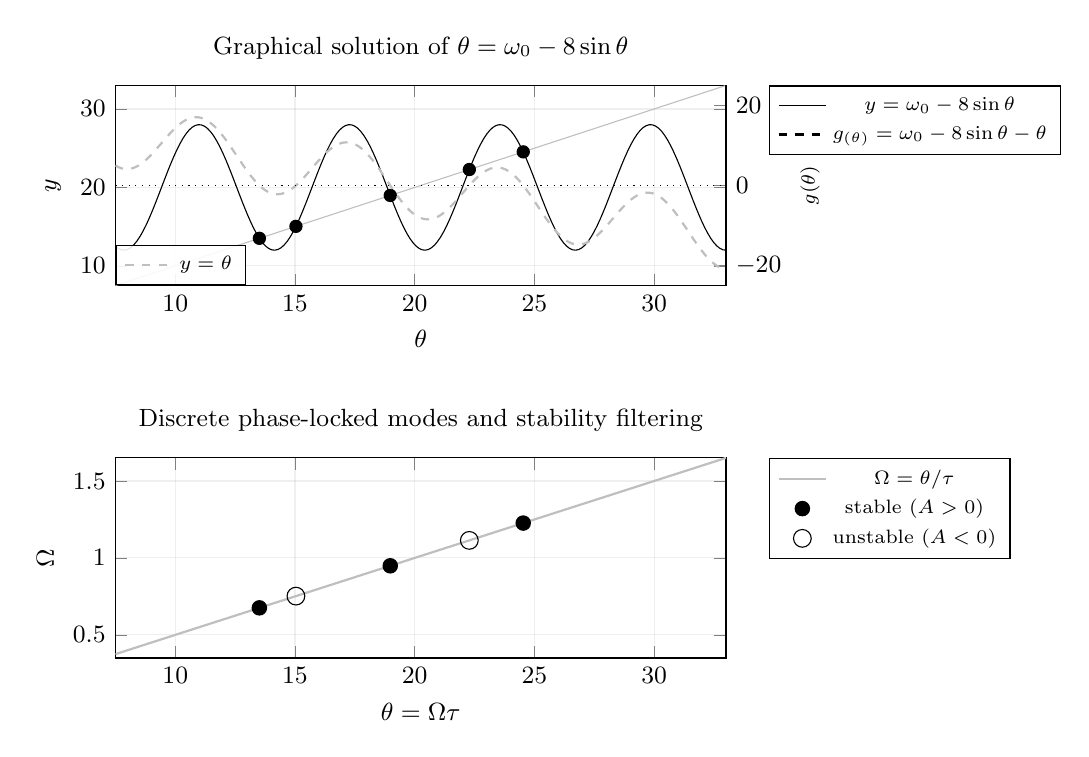
\begin{tikzpicture}
                \pgfplotsset{compat=1.18}

                % Parameters
                \def\wzero{20}     % omega0 = Omega0*tau
                \def\beta{8}       % beta  = K*tau
                \def\tauplot{20}   % tau

                % ========================
                % PANEL (a): main axis
                % ========================
                \begin{axis}[
                    name=panelA,
                    width=0.77\linewidth,
                    height=0.34\linewidth,
                    xmin=7.5, xmax=33,
                    ymin=7.5, ymax=33,
                    xlabel={$\theta$},
                    ylabel={$y$},
                    grid=major,
                    grid style={opacity=0.25},
                    tick label style={font=\small},
                    label style={font=\small},
                    title style={font=\small},
                    title={Graphical solution of $\theta=\omega_0-\beta\sin\theta$},
                    legend style={
                        draw=black, fill=white,
                        fill opacity=1, text opacity=1,
                        font=\scriptsize,
                        at={(1.07,1.00)}, anchor=north west  % legend outside right
                    },
                ]

                % y = omega0 - beta sin(theta)
                \addplot[black, domain=7.5:33, samples=200] {\wzero - \beta*sin(deg(x))};
                \addlegendentry{$y=\omega_0 -\beta\sin\theta$}

                % Legend entries for right-axis curves (declare here, plot on overlay axis)
                \addlegendimage{black,dashed,thick}
                \addlegendentry{$g_{(\theta)}=\omega_0 -\beta\sin\theta-\theta$}

                % intersections
                \addplot[only marks, mark=*, mark size=2.2pt, black]
                coordinates {
                    (13.51219,13.51219)
                    (15.03907,15.03907)
                    (18.97769,18.97769)
                    (22.28018,22.28018)
                    (24.53069,24.53069)
                };
                %\addlegendentry{intersections}

                % y = theta
                \addplot[white!75!black, domain=7.5:33, samples=200] {x};

                \end{axis}

                % ========================
                % PANEL (a): overlay right axis for g(theta)
                % ========================
                \begin{axis}[
                    at={(panelA.south west)}, anchor=south west,
                    width=0.77\linewidth,
                    height=0.34\linewidth,
                    xmin=7.5, xmax=33,
                    axis x line=none,
                    axis y line*=right,
                    ylabel={$g(\theta)$},
                    ymin=-25, ymax=25,               % adjust if needed
                    tick label style={font=\small},
                    label style={font=\scriptsize},
                    grid=none,
                    axis background/.style={fill=none},
                    legend style={
                        draw=black, fill=white,
                        fill opacity=0.9, text opacity=1,
                        font=\scriptsize,
                        at={(panelA.south west)}, anchor=south west,
                    },
                ]
                    \addlegendentry{$y=\theta$}
                    % g(theta) = omega0 - beta sin(theta) - theta   (NO "20+")
                    \addplot[white!75!black, dashed, thick, domain=7.5:33, samples=200]
                    {\wzero - \beta*sin(deg(x)) - x};

                    % zero line
                    \addplot[black, dotted, domain=7.5:33, samples=2] {0};

                \end{axis}

                % ========================
                % PANEL (b): spectrum
                % ========================
                \begin{axis}[
                    at={(panelA.below south west)}, anchor=above north west,
                    yshift=-0.55cm,
                    width=0.77\linewidth,
                    height=0.34\linewidth,
                    xmin=7.5, xmax=33,
                    ymin=0.35, ymax=1.65,
                    xlabel={$\theta=\Omega\tau$},
                    ylabel={$\Omega$},
                    grid=major,
                    grid style={opacity=0.25},
                    tick label style={font=\small},
                    label style={font=\small},
                    title style={font=\small},
                    title={Discrete phase-locked modes and stability filtering},
                    legend style={
                        draw=black, fill=white,
                        fill opacity=1, text opacity=1,
                        font=\scriptsize,
                        at={(1.07,1.00)}, anchor=north west  % legend outside right
                    },
                ]

                    % Omega = theta/tau
                    \addplot[white!75!black, thick, domain=7.5:33, samples=200] {x/\tauplot};
                    \addlegendentry{$\Omega=\theta/\tau$}

                    % stable points (A>0)
                    \addplot[only marks, mark=*, mark size=2.6pt, black]
                    coordinates {
                        (13.51219,0.675609)
                        (18.97769,0.948885)
                        (24.53069,1.226534)
                    };
                    \addlegendentry{stable ($A>0$)}

                    % unstable points (A<0)
                    \addplot[only marks, mark=o, mark size=3.2pt, black]
                    coordinates {
                        (15.03907,0.751954)
                        (22.28018,1.114009)
                    };
                    \addlegendentry{unstable ($A<0$)}

                \end{axis}

            \end{tikzpicture}

            \caption{\footnotesize
            Phase locking and stability filtering for the transcendental self-consistency equation
                $\theta=\omega_0-\beta\sin\theta$ (Eq.~\ref{eq:theta_beta}).
                (a) Intersections of $y=\theta$ and $y=\omega_0-\beta\sin\theta$ define phase-locked branches.
                The auxiliary function $g(\theta)=\omega_0-\beta\sin\theta-\theta$ (dashed, right axis) vanishes at the same points.
                (b) Corresponding frequencies $\Omega=\theta/\tau$ with stable branches ($A=K\cos\theta>0$) filled and unstable branches open.
            }
            \label{fig:phase_locking}
        \end{figure}

        \paragraph{Stability Filtering and the Characteristic Equation}

            Linearizing Eq.~\ref{eq:delayed_oscillator} about a phase-locked solution yields
            \begin{equation}
                \delta\dot{\phi}(t)
                =
                A\big(\delta\phi(t-\tau)-\delta\phi(t)\big),
                \qquad
                A=K\cos(\Omega\tau),
                \label{eq:linearized_phi}
            \end{equation}
            with characteristic equation
            \begin{equation}
                \lambda = A\left(e^{-\lambda\tau}-1\right).
                \label{eq:characteristic}
            \end{equation}

            The root $\lambda=0$ reflects global phase-shift invariance.
            Orbital stability requires all other roots satisfy $\Re(\lambda)<0$.

        \paragraph{Unconditional Stability for \texorpdfstring{$A>0$}{A>0}}

            Let $\lambda=u+iv$.
            Taking the real part of Eq.~\ref{eq:characteristic} gives
            \begin{equation}
                u=A\big(e^{-u\tau}\cos(v\tau)-1\big).
                \label{eq:real_part}
            \end{equation}

            Assume $A>0$ and suppose $u\ge0$.
            Since $e^{-u\tau}\le1$ and $\cos(v\tau)\le1$, it follows that
            \[
                e^{-u\tau}\cos(v\tau)-1 \le 0,
            \]
            hence $u\le0$.
            Thus the only possibility with $u\ge0$ is $u=0$, which requires $v=0$.
            All nontrivial eigenvalues satisfy $\Re(\lambda)<0$.
            Branches with $A>0$ are therefore unconditionally stable.

        \paragraph{Conditional Stability for \texorpdfstring{$A<0$}{A<0}}

            For $A<0$, set $\lambda=u\in\mathbb{R}$.
            Define
            \[
                f(u)=u-A(e^{-u\tau}-1).
            \]
            We have $f(0)=0$ and
            \[
                f'(0)=1+A\tau.
            \]

            If $A\tau<-1$, then $f'(0)<0$.
            Since $f(u)\to+\infty$ as $u\to+\infty$, a strictly positive real root exists.
            Hence instability occurs when
            \begin{equation}
                A\tau<-1.
                \label{eq:stability_window}
            \end{equation}

            The above argument establishes that
            \begin{equation}
                A\tau<-1
            \end{equation}
            is a sufficient condition for linear instability, since in that case a strictly positive real eigenvalue exists.
            A necessary condition for stability is therefore
            \begin{equation}
                A\tau\ge -1.
            \end{equation}

        \paragraph{Branch Selection for \texorpdfstring{$\beta\gg1$}{beta>>1}}

            At the approximate roots $\theta_m\approx m\pi$,
            \begin{equation}
                A_m\tau = K\tau\cos(m\pi) = \beta(-1)^m.
            \end{equation}

            \begin{itemize}
                \item Even $m=2n$: $A_{2n}\tau\approx\beta>0$.
                These branches satisfy $A>0$ and are unconditionally stable, as shown above.

                \item Odd $m=2n+1$: $A_{2n+1}\tau\approx-\beta$.
                In the strong-feedback regime ($\beta\gg1$), this gives $A\tau\ll-1$, which satisfies the sufficient instability condition derived above.
                Hence all odd-indexed branches are dynamically unstable.
            \end{itemize}

            Thus, in the regime $\beta\gg1$, stability filtering selects the even-indexed subset of branches,
            \begin{equation}
                \Omega_n\tau\approx2\pi n,
            \end{equation}
            yielding an evenly spaced integer-indexed family of dynamically stable modes.

    \paragraph{Branch Density}

        The uniform spacing $\Delta\Omega\approx2\pi/\tau$ implies a spectral density
        \begin{equation}
            \rho(\Omega)=\frac{dn}{d\Omega}\approx\frac{\tau}{2\pi},
            \end{equation}

        The branch density therefore scales linearly with delay length.
        The resulting spectrum reproduces the asymptotic spacing of boundary-value quantization without imposing spatial confinement.
    \section{Interpretation}
    The analysis demonstrates that finite propagation time alone is sufficient to generate discrete circulation modes through classical phase locking. Discreteness emerges at the level of delay--induced feedback dynamics, prior to the introduction of any additional structural constraints. In circulation--based theories, geometric or topological features may enhance the robustness and longevity of selected modes, but they are not responsible for their initial appearance.

    From this perspective, discrete mode families should be regarded as a generic feature of scalar phase oscillators with delayed self-interaction rather than a peculiarity of specific physical realizations. The mechanism applies equally to optical cavities, electronic delay lines, mechanical rotors, and fluid circulation systems whenever delayed self--interaction is present.

    \section{Conclusion}
    Phase locking in closed loops with finite circulation time provides a universal and purely classical mechanism for discrete mode selection. Any scalar circulating system with delayed self--interaction of the form considered here generically admits a discrete set of dynamically stable phase--locked states. This framework offers a conservative and analytically tractable foundation for understanding mode discreteness in a wide range of physical systems governed by delayed feedback, and it clarifies how discrete behavior can arise naturally from continuous classical dynamics.

    \section*{Declarations}

        \subsection*{Funding}
            The author received no specific funding for this work.

        \subsection*{Conflict of interest}
            The author declares that there is no conflict of interest.

        \subsection*{Data availability}
            No datasets were generated or analyzed during the current study.

        \subsection*{Author contributions}
            Omar Iskandarani solely conceived the study, developed the model, performed the analysis, and wrote the manuscript.

%=========================================
% References
%=========================================
    \bibliographystyle{unsrt}
    \begin{thebibliography}{99}
        \bibitem{Erneux2009} Erneux, T. (2009). \textit{Applied Delay Differential Equations}. Springer, New York. DOI: 10.1007/978-0-387-74372-1

        \bibitem{Earl2003} Earl, M. G., \& Strogatz, S. H. (2003). Synchronization in oscillator networks with delayed coupling: A rigorous proof. \textit{Physical Review E}, 67(3), 036204. DOI: 10.1103/PhysRevE.67.036204

        \bibitem{Hale1993} Hale, J. K., \& Verduyn Lunel, S. M. (1993). \textit{Introduction to Functional Differential Equations}. Springer, New York.

        \bibitem{Diekmann1995} Diekmann, O., van Gils, S. A., Verduyn Lunel, S. M., \& Walther, H.-O. (1995). \textit{Delay Equations: Functional-, Complex-, and Nonlinear Analysis}. Springer, New York.

        \bibitem{GlassMackey1988} Glass, L., \& Mackey, M. C. (1988). \textit{From Clocks to Chaos: The Rhythms of Life}. Princeton University Press, Princeton.

        \bibitem{Ikeda1979} Ikeda, K. (1979). Multiple-valued stationary state and its instability of the transmitted light by a ring cavity system. \textit{Optics Communications}, 30(2), 257--261. DOI: 10.1016/0030-4018(79)90090-7

        \bibitem{Kuramoto1984} Kuramoto, Y. (1984). \textit{Chemical Oscillations, Waves, and Turbulence}. Springer, Berlin.

        \bibitem{Pikovsky2001} Pikovsky, A., Rosenblum, M., \& Kurths, J. (2001). \textit{Synchronization: A Universal Concept in Nonlinear Sciences}. Cambridge University Press, Cambridge.

        \bibitem{Strogatz2003book} Strogatz, S. H. (2003). \textit{SYNC: The Emerging Science of Spontaneous Order}. Hyperion, New York.

        \bibitem{Gardner2005} Gardner, F. M. (2005). \textit{Phaselock Techniques} (3rd ed.). Wiley, Hoboken.

        \bibitem{Zettl2005} Zettl, A. (2005). \textit{Sturm--Liouville Theory}. American Mathematical Society, Providence.

        \bibitem{Griffiths2018} Griffiths, D. J., \& Schroeter, D. F. (2018). \textit{Introduction to Quantum Mechanics} (3rd ed.). Cambridge University Press, Cambridge.

        \bibitem{Siegman1986} Siegman, A. E. (1986). \textit{Lasers}. University Science Books, Mill Valley.
    \end{thebibliography}

\end{document}